The DrK is an attack against KASLR which derandomizes the kernel address space.
It has been proposed in the paper \textit{Breaking Kernel Address Space Layout Randomization with Intel TSX} by \textit{Jang, Yeongjin and Lee, Sangho and Kim, Taesoo} \cite{drk}.
Most of the code necessary to perform the attack can be found on \href{https://github.com/sslab-gatech/DrK}{GitHub} \cite{drk-attack-proof-of-concept-github}.

The attack builds upon Intel TSX and performs a timing attack to infer the state of a page (mapped vs. unmapped and executable vs. non-executable).
This works because with TSX the kernel does not get notified of Page Faults and Access Violations, but the abort handler itself is.
Furthermore the time it takes the \textit{MMU} (Memory Managment Unit) to throw a Page Fault exception slightly differs from the time it takes to throw an Access Violation exception.
Using this the status of a page can be inferred.\cite{drk}

\subsection{Intel TSX}

Intel TSX stands for the Intel Transaction Synchronization Extension(s) \cite{intel-tsx-overview}.
It is an interface using which code can be run transactionally, i.e. segmented into clearly defined transactions, aborted and rolled back including all memory writes if so desired.

Aborting and rolling back happens either manually using a directive to abort the transaction or automatically in the case of an exception such as a Page Fault.

\lstset{language=C, basicstyle=\small\ttfamily,
        string=[b]', showspaces=false, showtabs=false,
        caption={Example code for Intel TSX}, captionpos=b}
\begin{lstlisting}
// start transaction, if rolled back
// execution continues from here
// but with a different return value
// (status code of transaction)
if (_xbegin() == _XBEGIN_STARTED) {

  ... // do work

  // commit transaction
  _xend();

  // or abort with status code
  // (=> rollback)
  _xabort(status)
} else {
  // abort handler
}
\end{lstlisting}

The exception being directly handled by an abort handler in userspace is far from the norm. Otherwise this will always notify the kernel which can then decide to terminate the process or take some other kind of action.
With TSX this is not possible as the kernel does not ever get notified of this exception occuring.
This can pose great potential for abuse if used in a nefarious manner as this behavior differs from the status quo and assumptions used elsewhere might not hold with this.
Mechanisms which otherwise rely on the kernel getting notified about page faults such as Demand Paging will not work correctly.\cite{drk}

\subsection{Timing differences}

The abort handler does not get information about what exception occured.
Page Faults point to the page being unmapped, while Access Violations point to the page being mapped but inaccessible from userspace.
Differentiating a Page Fault from an Access Violation will have to be done in some other way.
The time the MMU needs to generate a Page Fault for a given memory access differs from the time it takes to generate an Access Violation as the prior one can be deduced faster.
This difference can be measured and used to tell both apart.\cite{drk}

Checking for the execution status of the page works similarly.
For a page that is known to be mapped (but inaccessible from userspace, meaning it belongs to the kernel address space) trying to jump to an address contained in the page will take a different amount of time until the exception is generated based on whether the page is executable or not.\cite{drk}

\subsection{Crafting the attack}

Combining the previous leads to the following exploit implementation.

By reading from a memory address a Page Fault will be generated if the page is unmapped and an Access Violation if the page is mapped but inaccessible from userspace.
To achieve this, inline assembly is used to move the value at the given address into a register, i.e. a very simple method to read from a concrete memory address.

This function will be called for each page and the timing results interpreted afterwards.

\lstset{language=C, basicstyle=\small\ttfamily,
        string=[b]', showspaces=false, showtabs=false,
        caption={Mapped vs Unmapped timing test{\cite[Figure~3]{drk}}}, captionpos=b}
\begin{lstlisting}
uint64_t do_probe_mapped(void* addr) {
  // start timer
  uint64_t beg = rdtsc_beg();

  if (_xbegin() == _XBEGIN_STARTED) {

    // generates access violation
    // mapped vs unmapped
    asm volatile("mov rax, [addr]");
  } else {
    // compute time difference
    return rdtsc_end() - beg;
  }
}
\end{lstlisting}

Similarly the code can be adapted slightly to check for the execution status of a page.
Here instead of reading from an address we try to jump to it.

\lstset{language=C, basicstyle=\small\ttfamily,
        string=[b]', showspaces=false, showtabs=false,
        caption={Executable vs Non-Executable timing test{\cite[Figure~3]{drk}}}, captionpos=b}
\begin{lstlisting}
uint64_t do_probe_executable(void* addr) {
  // start timer
  uint64_t beg = rdtsc_beg();

  if (_xbegin() == _XBEGIN_STARTED) {

    // generates access violation
    // executable vs non-executable
    asm volatile(
      "mov rax, addr; jmp rax"
    );
  } else {
    // compute time difference
    return rdtsc_end() - beg;
  }
}
\end{lstlisting}

\subsection{Interpreting the results}

Using \lstinline{do_probe_mapped} and \lstinline{do_probe_executable} the status of a page can be inferred.
To do so the functions are called multiple times and the minimum time is recorded.

\lstset{language=C, basicstyle=\small\ttfamily,
        string=[b]', showspaces=false, showtabs=false,
        caption={Collect timing results{\cite[Figure~3]{drk}}}, captionpos=b}
\begin{lstlisting}
uint64_t probe_memory(
  int ntimes,
  int (*do_probe_memory)(void*),
  void* addr
) {
  uint64_t min = UINT64_MAX;
  while (ntimes --) {
    uint64_t clk = do_probe_memory(addr);
    // Only record the minimum
    // timing observed.
    if (clk < min)
      min = clk;
  }
  return min;
}
\end{lstlisting}

Testing with known mapped pages, executable pages as well as unmapped and non-executable pages leads to the following results being shown in \autoref{fig:timing_m_u} and \autoref{fig:timing_x_nx}.

\begin{figure}[h]
  \begin{center}
    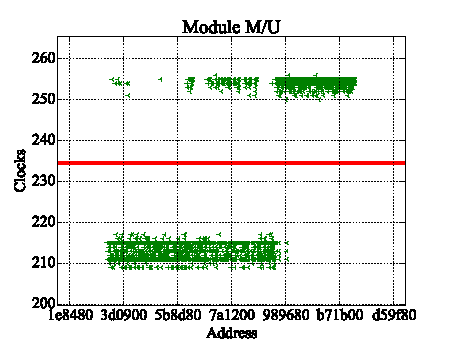
\includegraphics[page=1,width=.4\textwidth]{fig/prebuilt_results_M_U}
  \end{center}
  \caption{Mapped vs Unmapped \cite[Figure~6]{drk}}
  \label{fig:timing_m_u}
\end{figure}

\begin{figure}[h]
  \begin{center}
    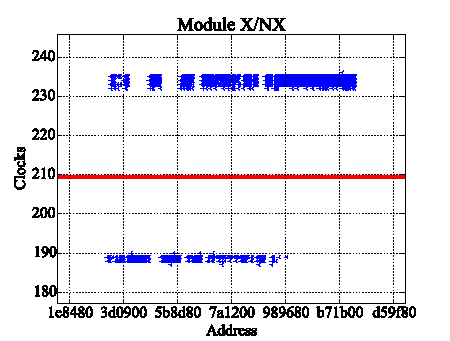
\includegraphics[page=1,width=.4\textwidth]{fig/prebuilt_results_X_NX}
  \end{center}
  \caption{Executable vs Non-Executable \cite[Figure~6]{drk}}
  \label{fig:timing_x_nx}
\end{figure}

Very clear-cut groupings can be observed, using those a categorization into (M)apped vs (U)nmapped and Executable (X) and Non-Executable (NX) can be done.
These values are dependent on the CPU being used. Different hardware will have different timing thresholds.

\begin{figure}[h]
  \begin{center}
    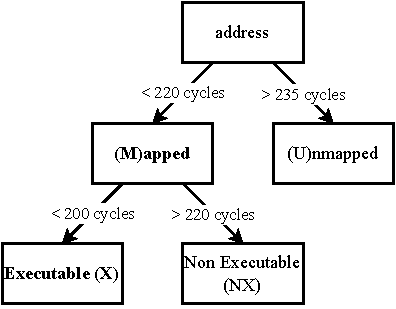
\includegraphics[page=1,width=.4\textwidth]{fig/prebuilt_decision_tree}
  \end{center}
  \caption{Decision tree for categorization of pages\cite[Figure~4]{drk}}
  \label{fig:decision_tree}
\end{figure}

All read accesses which take less than 220 cycles are considered to be mapped.
Accesses which take more than 235 cycles are considered to be unmapped.
For all pages considered to be mapped an additional check for their execution status is performed.
If jumping to the address takes less than 200 cycles the page is considered executable.
More than 220 cycles is considered non-executable.\cite{drk}

\subsection{Determining kernel and module mappings}

With the previous steps the status of a page can be inferred.
This however does not tell anything about what this page is actually being used for.
In many cases extra information such as the precise kernel location or the location of a specific module is required.
Thus a further step is necessary.

The general approach is to associate each known module as well as the kernel itself with a signature and then search the pool of pages for these signatures.
It is to be noted that a module or the kernel itself consists not only of a single page but multiple.

For this operating system specific rules and ranges for page allocation can be used to guess which page corresponds to which module or kernel region.

\subsubsection{Linux}

The address ranges into which the kernel and the modules are mapped are different and do not overlap.
It is therefore easy to tell kernel and module pages apart.
The kernel is located in the range \lstinline{[0xffffffff80000000, 0xffffffffc0000000)}.
Modules are mapped in the range \lstinline{[0xffffffffc0000000, 0xffffffffc0400000]}, thus directly following the address range of the kernel.

Similar to the kernel each module is also mapped as a continoues range of pages, but there is a gap comprised of empty pages in between each module's pages.
Knowing the amount of modules (exposed by \lstinline{lsmod}) and their sizes makes it possible to uniquely identify some of the modules \cite{drk}.

\subsubsection{Windows}
Unlike Linux Windows does not seperate the kernel and the modules into different address ranges.
Both are mapped into the range \lstinline{[0xfffff80000000000, 0xfffff80400000000]}.

Windows sets execute permissions on kernel pages, has at most 6 kernel pages, each with a size of 2MB.
Either the kernel comes before all drivers or after all drivers.

Scanning for the kernel is done by looking for 6 consecutive pages with execute permissions.
After that the location of the modules is either in front or behind the kernel.\cite{drk}

Windows does however have one more trick up its sleeves: The starting position of the kernel is randomized within the page itself.
Figuring out the page is not enough to correctly determine the location of functions or specific instructions.\cite{blog-windows-10-kaslr}

\subsubsection{macOS}

The kernel is mapped in the range \lstinline{[0xffffff8000000000, 0xffffff8020000000]}.
It can be found by looking for the first mapped page.\cite{drk}
